\chapter{The bridge}
In section \ref{sec:knowledge} is discussed, how situation awareness is created by monitoring the vessel. The crew monitors the vessel from the bridge. The development of the bridge design is driven by technological advancement and regulatory demands. Which has increased the amount of equipment on a ship's bridge. Leading to all different components giving more and more data. As described by Speier are nowadays new technologies the primary reason for information overload. Not only because it produces more data, more quickly. But also that this information is disseminated more easily to people who do not need it \cite{Speier1999}. 
This chapter goes a level deeper than the previous one. The focus is on the crew at the bridge, what instruments and equipment there is, how the bridge developed and might develop in the future. The chapter will be concluded with a part on the manoeuvring display which is most relevant for this research. 

\section{User stories crew}
To get insight into what the crew does on board of the ship, and which functions are desired. Different user stories will be written. In section \ref{sec:deck-crew} the different deck crew members with their responsibilities are already described. 
A user story has as main goal to define a measurable function. It might replace a list of requirements. The main focus is who, what and why. Not how it should be implemented or developed. Examples of these user stories related to the tool and model can be:
\begin{itemize}
	\item As a master I want to see within a few seconds if there are hazards, so that I can decide if I should pay extra attention.
	\item As a crew member I want to have a guarantee that I know about all hazards, so that I can make the right decision.
	\item As a navigator I want to be able to see the consequences of a decision, so that I can make the right consideration for future decisions.
	\item As a master I want to get extra information on relative speed and possible place of colliding, so that I can judge myself if there is a high risk.
	\item As a master I want to be able to communicate an explanation for our current status and the decisions we made, to port authorities, nearby vessels and other crew members, so that there is a shared mental model.
\end{itemize}
During the project, a list of these user stories will be formed, also based on conversations with crew members. Beside this, the different steps in the thought process should be mapped. Together with the user stories, this can be used to develop a good mental model of the different crew members. 
Thereby will I also try to consider communication between authorities, other vessels, pilots and within the ship during hand-overs. 

During this process, there will be three categories of information: relevant information, unused information, missing information. The unused information might lead to information overload. As Sandhaland already mentioned how information overload is one of the main reasons for loss of situation awareness. During the previously mentioned accidents was the desired information available. It was however, not interpreted correctly by the crew.

\newpage
\section{Bridge elements}
The bridge of a vessel has four elements according to DNV-GL. The human operator, procedures, technical system and the human-machine interface. The safe operation of the vessel can only be assured when these are aligned. In figure \ref{fig:Bridge-system-elements} the different elements and their key factors are shown. Regulations aim to regulate these factors to ensure a safe performance of the bridge system to ensure system reliability in various modes of operation under different operating conditions. \cite{DNVGL2011}
\begin{figure}[H]
	\centering
	\includegraphics[width=0.4\textwidth]{Bridge-system-elements.png}
	\caption{Bridge system elements}
	\label{fig:Bridge-system-elements}
\end{figure}

\section{Instruments and equipment}
Depending on the different station at the bridge certain equipment must be installed and within reach. But at least the following instruments and equipment shall be installed: navigation radar with radar, propulsion control, manual steering device (with take-over), heading control, \ac{ECDIS}, steering mode selector switch, \ac{VHF} unit, whistle and manoeuvring light push buttons, internal communication equipment, central alert management system \ac{UID}s, general alarm control, window wiper and wash controls, control of dimmers for indicators and displays, steering \ac{UID}s, propulsion, emergency stop for propulsion machinery, gyrocompass selector switch and steering gear pumps.

These different systems have indicators with information on: propeller revolution, speed over ground, windspeed and direction, rudder angle, rate-of-turn, heading, steering mode, steering position in command, depth indicator, clock, \ac{CAM-HMI}, alarm panel related to unmanned machinery space, alarm panel related to steering control system and steering gear, sound reception display and warning of surveillance period elapsing. 

Depending on the vessel some extra instruments can be for track control, steering control station selection, thruster \ac{UID}s and emergency stop for thrusters. Which give information on the thrust, pitch and when provided a conning information display  \cite{DNVGL2017}. Different examples of bridge designs can be found in figure \ref{fig:bridge-example}.

\begin{figure}[H]
	\centering
	
	\begin{subfigure}[b]{0.45\textwidth}
		\includegraphics[width=\textwidth]{brug-alphatron.jpg}
		\caption{Alphatron AlphaBridge}
	\end{subfigure}
	\hfill
	\begin{subfigure}[b]{0.45\textwidth}
		\includegraphics[width=\textwidth]{Brug-ASD-2310-PATRIOT.JPG}
		\caption{DAMEN ASD Tug 2310 (Patriot)}
	\end{subfigure}
	\hfill
	\begin{subfigure}[b]{0.45\textwidth}
		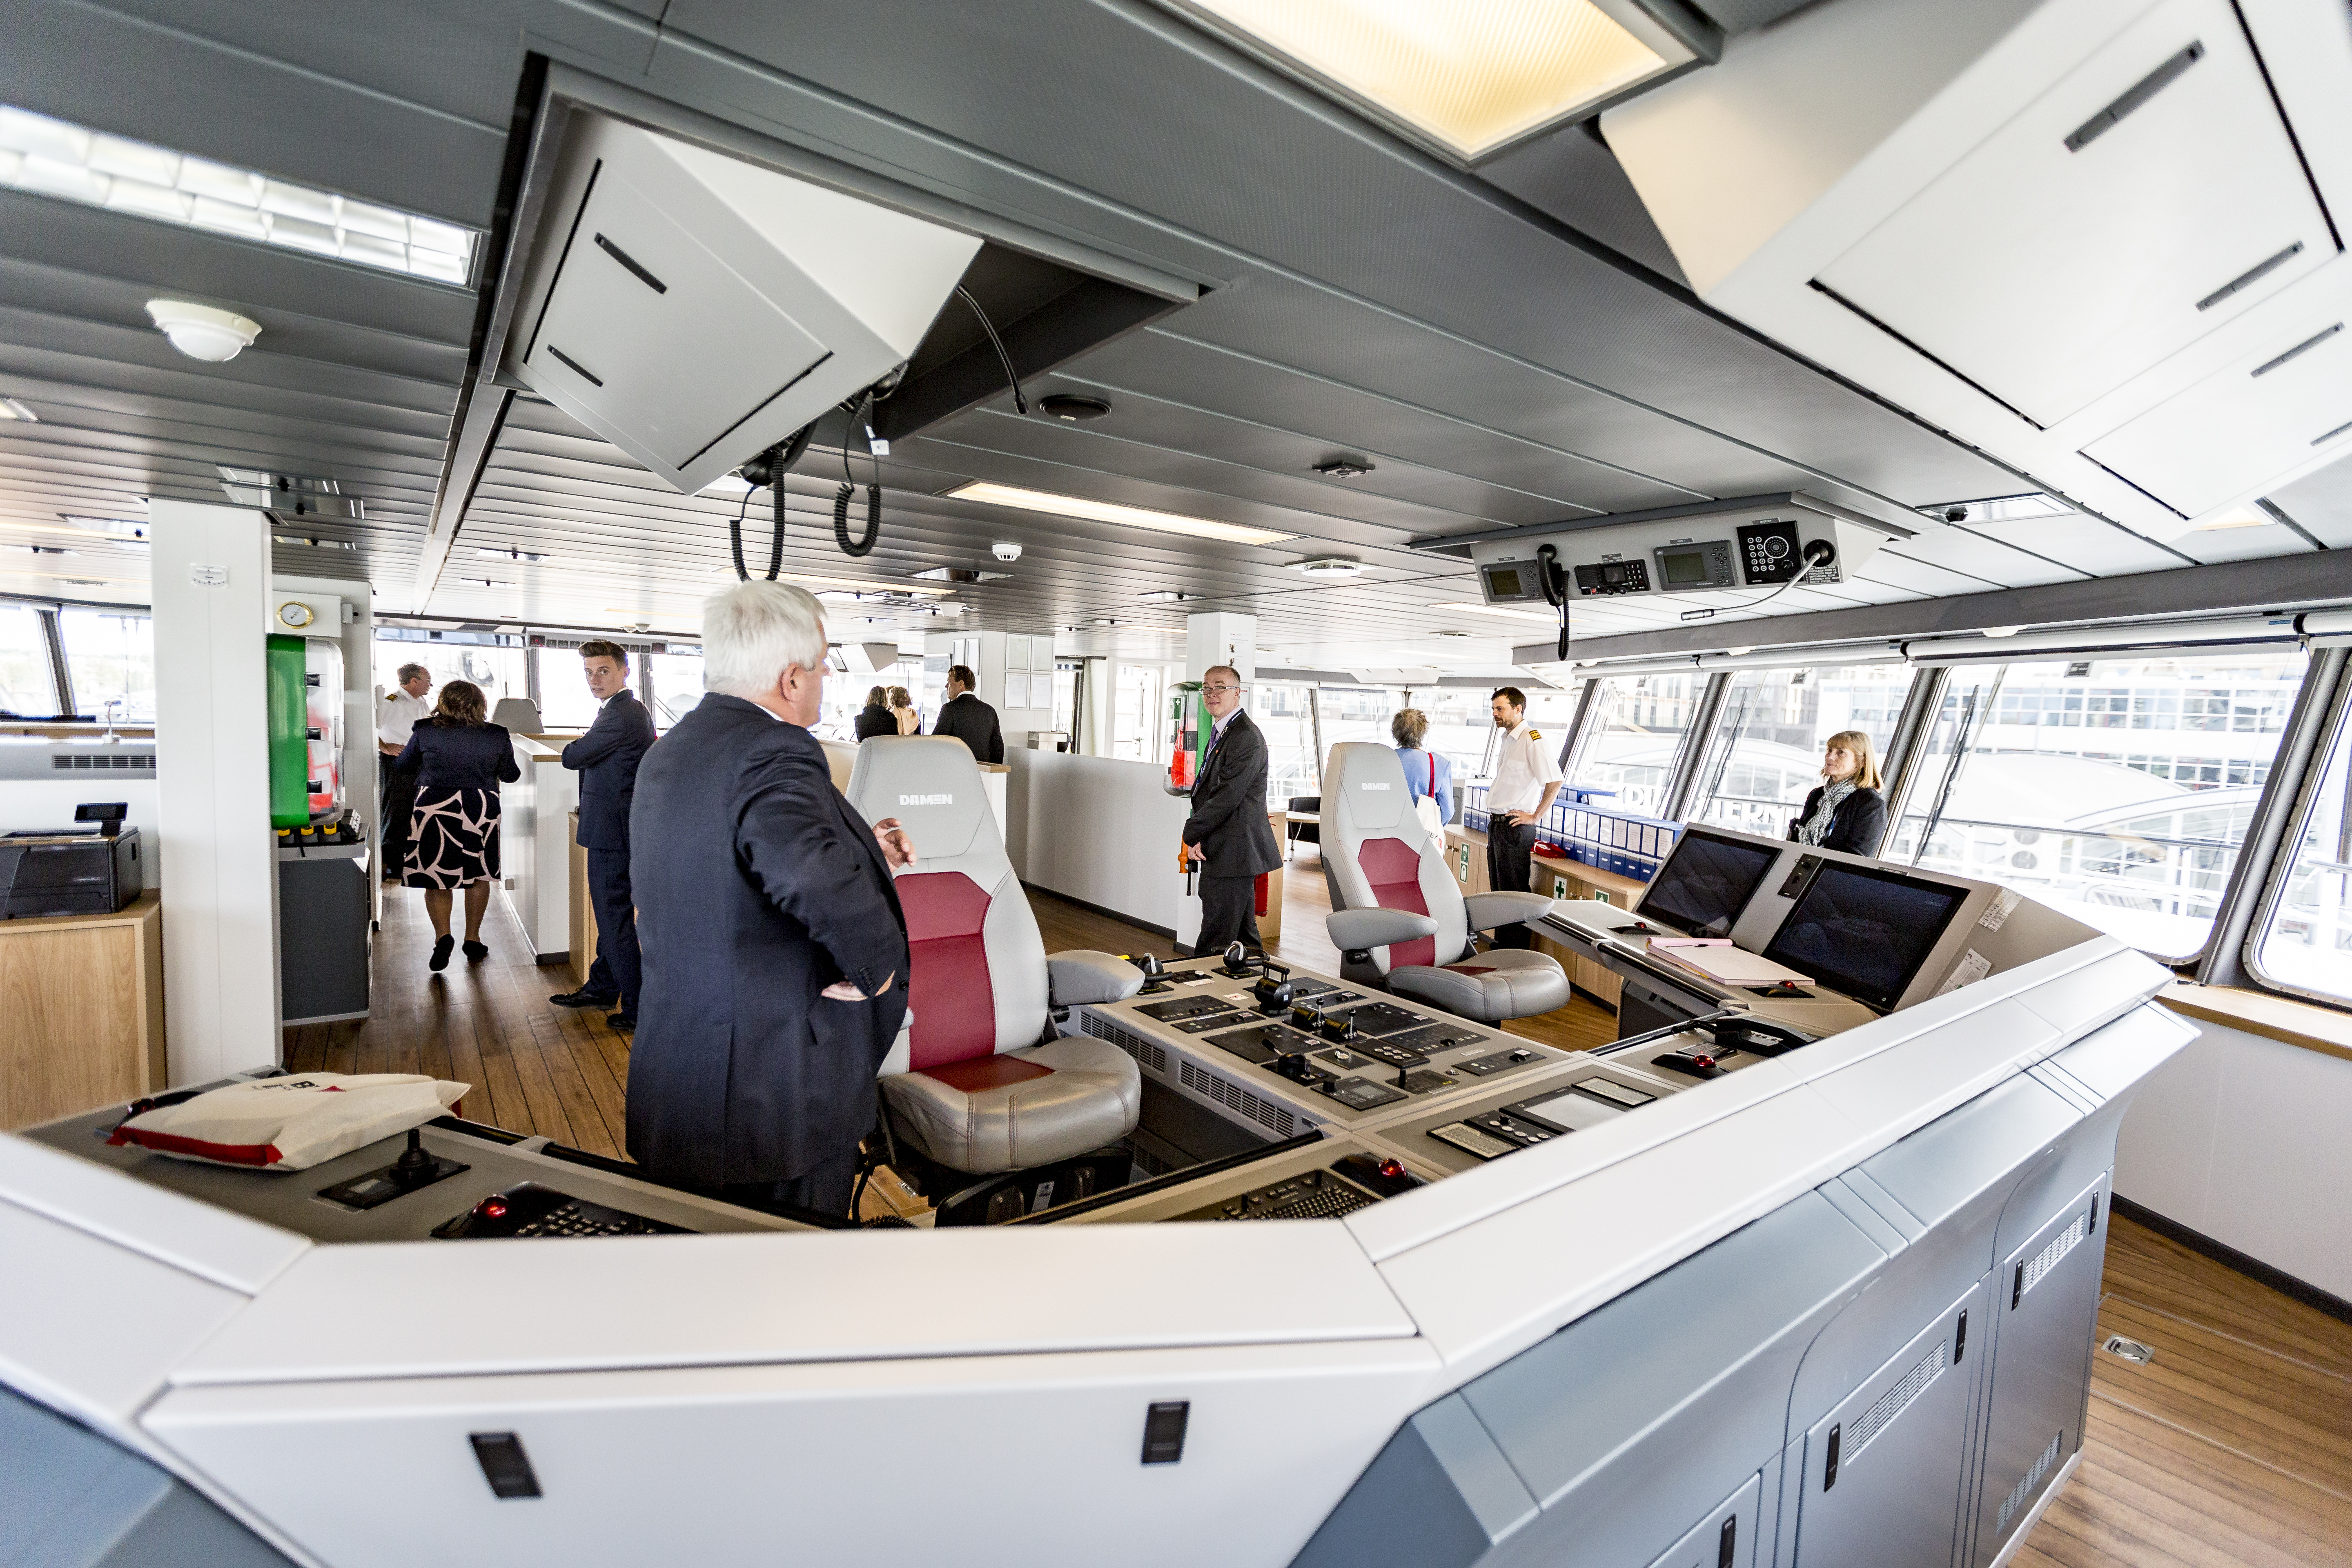
\includegraphics[width=\textwidth]{Brug-Bibby-Wavemaster.jpg}
		\caption{BIBBY WAVEMASTER 1}
	\end{subfigure}
	\hfill
	\begin{subfigure}[b]{0.45\textwidth}
		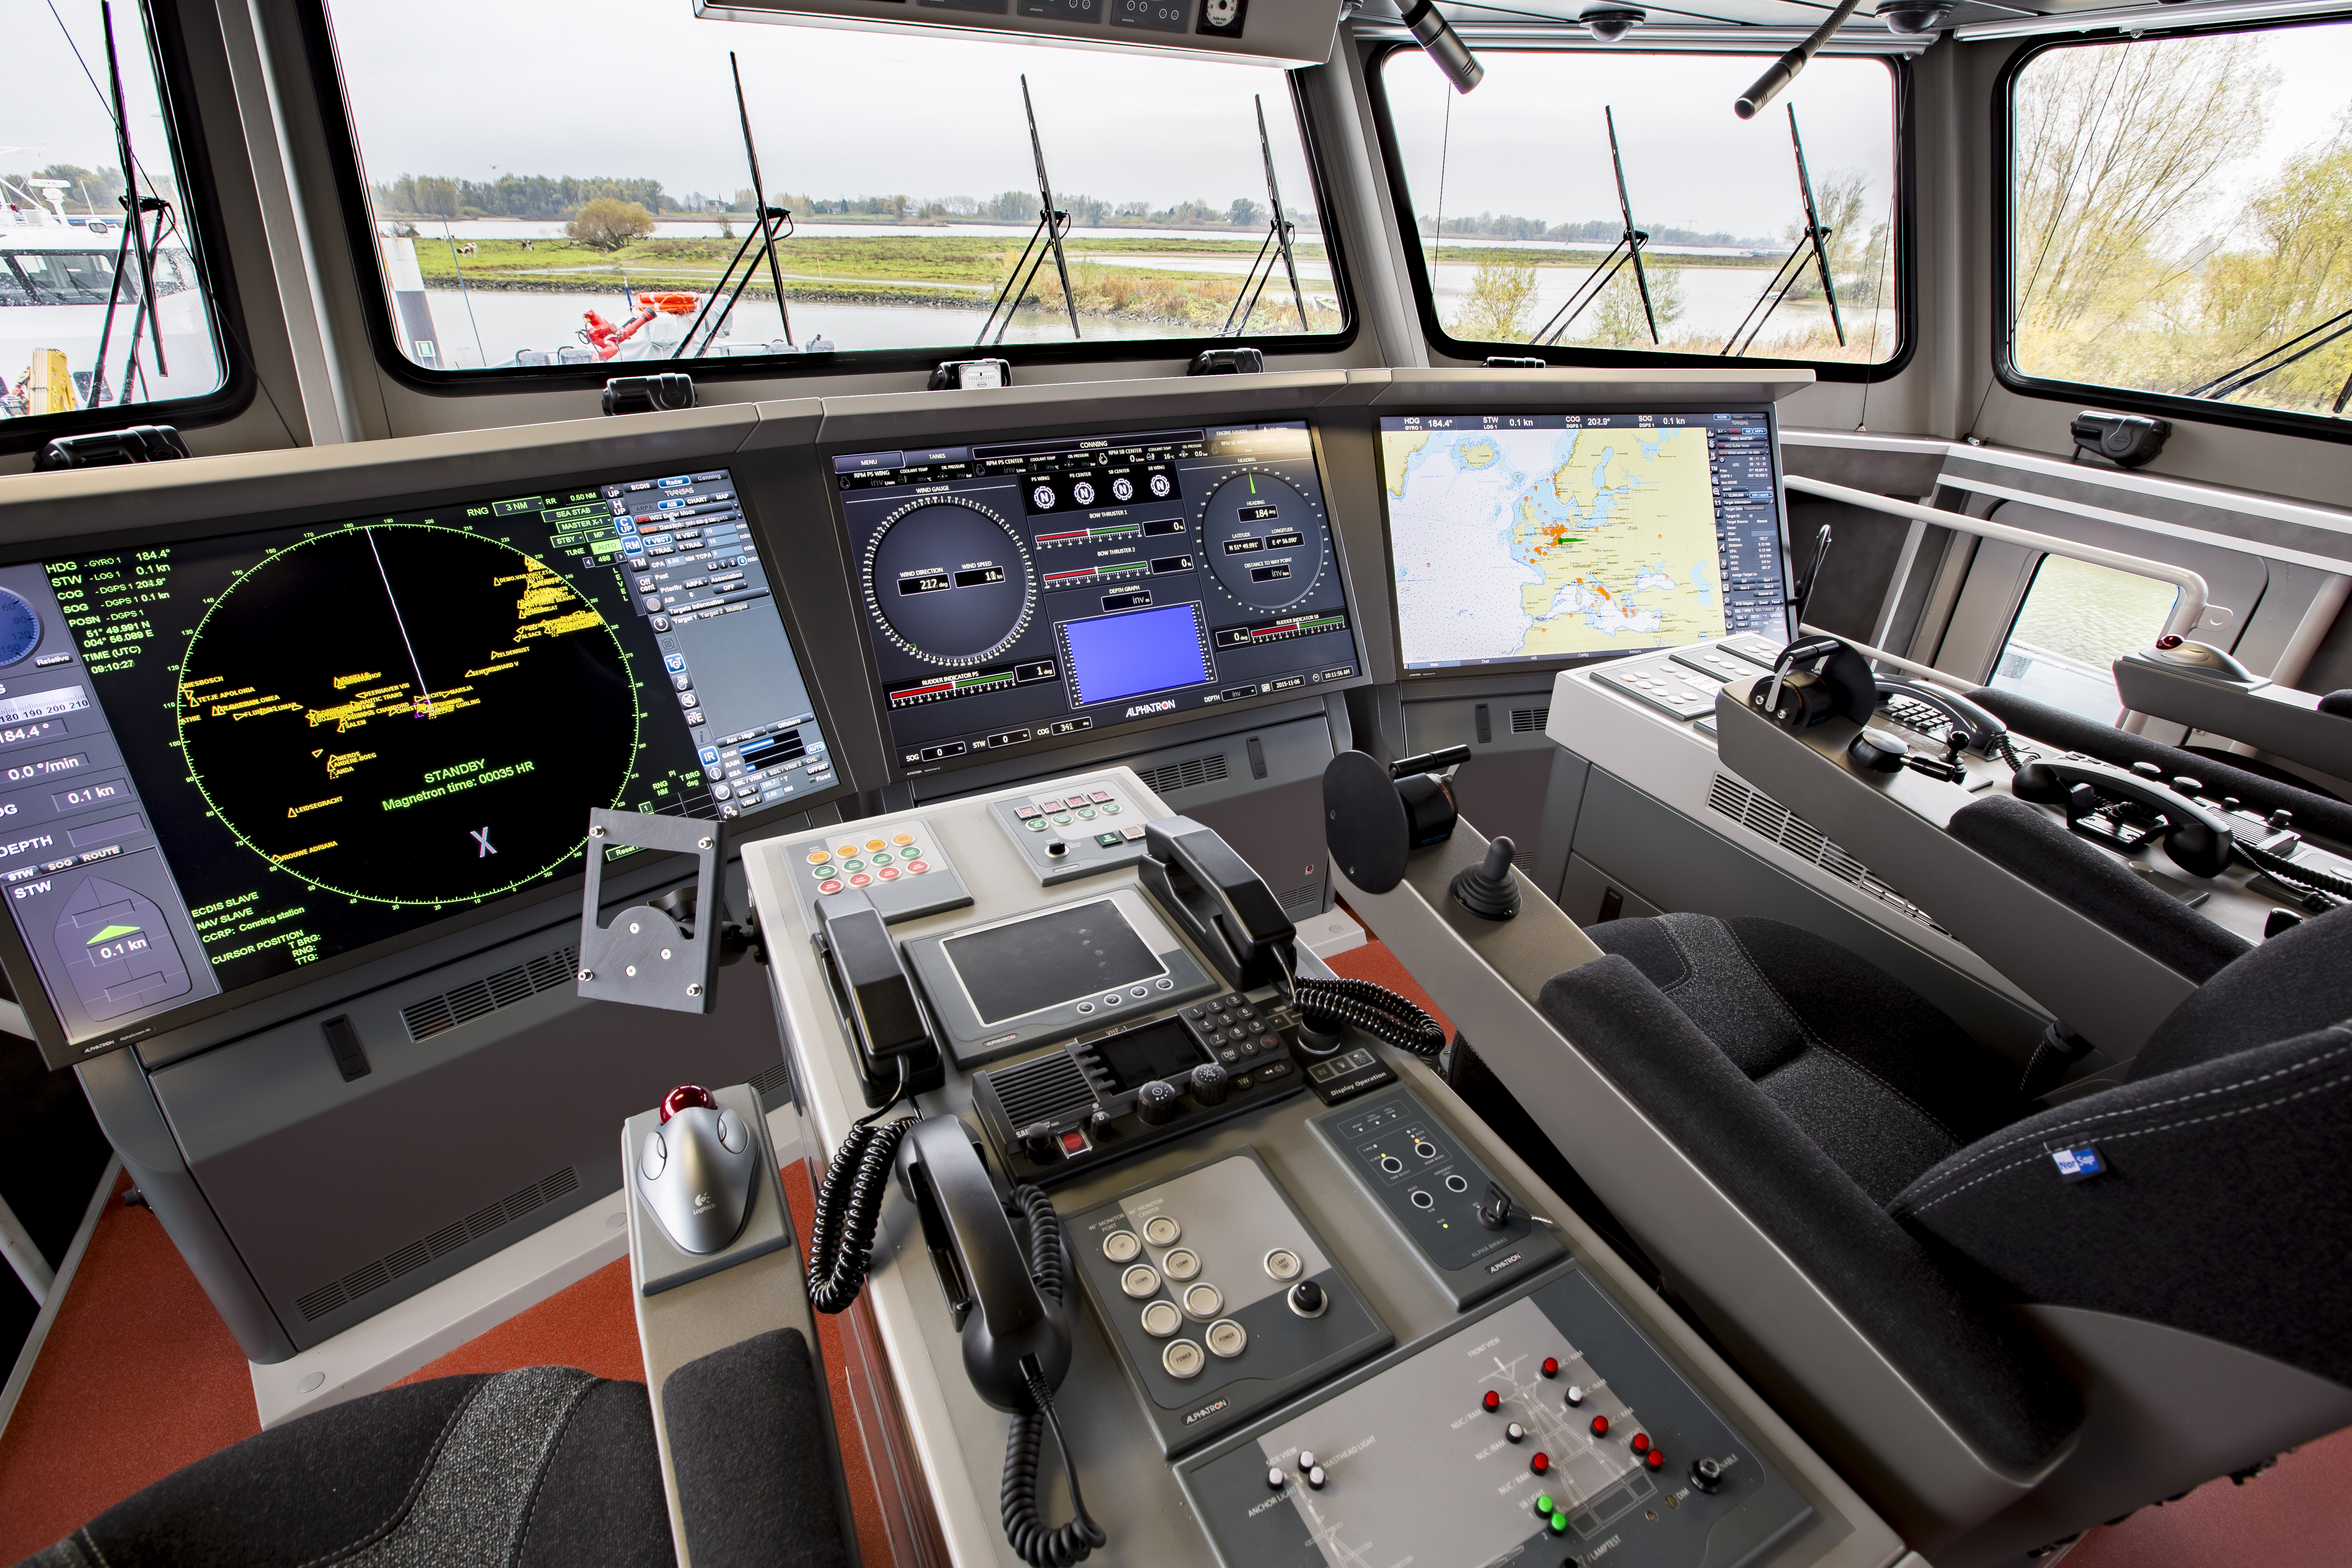
\includegraphics[width=\textwidth]{Brug-SPa-5009-Trinidad.jpg}
		\caption{DAMEN Stan Patrol 5009}
	\end{subfigure}	
	
	\caption{Various examples of bridge designs}
	\label{fig:bridge-example}
	
\end{figure}

\section{History of bridge design}
A brief history of bridge design starts at the transition from sailing ships to paddle steamers in the 19th century. Where the captain's sight could not be obstructed by the paddle houses, and engineers needed a platform from which they could inspect the paddle wheels. A raised walkway was created between both paddle houses, literally a bridge. The name bridge stuck, even when ships started using screw propellers. From the bridge, commands were passed via officers to the different stations. Where physical actions were carried out to control the ship. As technology did not exist to remotely control the ship. The helmsman or coxswain operated the ship's wheel from the enclosed wheelhouse, and engineers received commands in the engine room via engine order telegraphs. Where the bridge was often open to the elements, a weatherproof pilot house could be provided, from which the navigation officer could issue commands.

With the development of steel ship, came also the requirement of a compass platform. Sited as far away as possible from ferrous interference. Later this was solved with a binnacle. But this was another system which was introduced. In modern vessels, most of the stations for physical control have been moved to the bridge. The rudder and throttle can be operated directly from the bridge. Due to previous accidents, it is even common to have unmanned machinery spaces during operation in smaller ships. The technological developments have also lead to a variety of systems as mentioned above. Starting with radar at the start of the 20th century. \ac{ECDIS} was another major step forward, where it was accepted in 1995 by IMO as an up-to-date chart as required by \ac{SOLAS}. Later made mandatory in 2009 by \ac{SOLAS}, where \ac{STCW} requires \ac{ECDIS} competence for navigational officers and masters. This added an extra screen. Continuously adding other instruments for meteo, \ac{AIS}, echo sounder, different compasses, etc. First, the different instruments had all a separate analog instrument. Nowadays these are often displayed together at the conning display. While having the separate instruments at less convenient places.

\section{Future of bridge design}
This conning display already gave the opportunity to develop a more user oriented-bridge environment. But with the continuous development of different sensors. A new revolution is coming for bridge design using among others: sensor fusion, new ways of visualization and decision support. These are known as integrated bridge systems.
The development of future bridge designs goes parallel to the research into autonomous vessels. Both can be traced back to the changes in philosophy on human-computer interaction. Below some of the concepts are explained where often a combination of classification societies, research institutes, and commercial companies are involved.

\subsection{Concept designs}
Within Damen, there is the desire to make the bridge design more standard and create more of a brand identity. An integrated design is desired in this case, where suppliers deliver the back-end. Similar projects which already show a future vision of ship design are the Ulstein Bridge Vision concept and Rolls Royce oX bridge. Where augmented reality in the windows and adapting user interfaces are key. With early warnings, decision support for economic sailing, environmental analysis, and having the ability to use the windows as a screen to simulate operations. While it is clear that here lies the future of bridge design, they did not yet come with clear solutions. Although in projects like Waterborne some steps are made when it comes to the user interface.\cite{RollsRoyce2015} \cite{Ulstein2013}

\subsection{Research projects}
The CASCADe project has already been more research-oriented and towards a practical solution. They have tried to develop a bridge system which adapts displayed content on the user interfaces to the current situation, relevant procedures and the needs of the crew. Using a virtual simulation platform which enables analysis of the cooperative bridge system purely based on models, in particular, Cognitive Seafarer Models which mimic decision making and situation awareness processes of real human seafarers. The virtual platform allows a very careful evaluation of the Adaptive Bridge System to research solutions for adaptation which provide benefits (e.g., increase situation awareness) that outweigh their costs (e.g. cognitive disruption).\cite{CASCADe2015}
Within Damen there has been research on bridge design by Myrthe Lamme. She looked into the development of an identifiable, integrated, and user-focused bridge concept. She did this from an industrial design perspective. Her focus kept in mind the current information, and how this can be presented. But did not really look into presenting different information on hazards for example.

%\todo{add information on JIP which Robert presented, inlcuding the flowchart, if my project is able to use the same philosophy}

\subsection{Suppliers}
But currently bridges are already built and the companies developing these are also not standing still. But present more realistic their current status. The Kongsberg K-Master work environment integrates already different systems in one user interface. Dynamic positioning, manual propulsion and thruster control, alarm monitoring and remote control of machinery, central bridge alarm system, the operation of auxiliary bridge systems and chart, radar, autopilot and conning displays are all combined. Where this system was originally only for the aft bridge, is it now used for a variety of vessels. \cite{Kongsberg2017}
Many of the Damen vessels are making the step towards integrated bridge systems, which is the next step in a more user-centered design. Examples are, Praxis' Mega-Guard IBS or Alphatron's AlphaBridge. On a single screen Radar, ECDIS, conning, alarms, other ship systems and AIS can be combined. 
Other major players in the development of integrated bridge designs are Sperry Marine, Raytheon Anschütz and Admarel.

\section{Manoeuvring display}
The CASCADe project already showed the advantages of an adaptive bridge system. This is among other things done by creating an overlay in the \ac{ECDIS}. Which is a geographic information system used for nautical navigation. It displays information from \ac{ENC}. And integrates position information, heading and speed through water. Possibly add radar and \ac{AIS} information. Using alarms when the vessel gets in proximity to hazards. 

For this project, an overlay will be created to the \ac{ECDIS}. Which improves the current alarm system. Using a white box approach in the model will help to define alarms and mark forbidden zones. Which forms the overlay for the \ac{ECDIS}.
Thereby need to be taken into account, the rules and regulations for the \ac{ECDIS} system as defined by the \ac{IHO} and \ac{IEC} based on \ac{IMO} resolutions. Three important standards are IEC 61924-2:2012, IEC 61174:2015 and IEC 62065:2014.
The first specifies the minimum requirements for the design, manufacture, integration, methods of testing and required test results for an integrated navigation system.
The second specifies the performance requirements, methods of testing and required test results of the \ac{ECDIS}.
The third specifies the minimum requirements for track control systems, including alarms and warnings.
To understand how this information can be added, more information on the backend is needed. The \ac{IHO} standard for \ac{ENC} datasets is S-57. Which normally have a .000 extension. Update files for the \ac{ENC} have extensions like .001, .002 and so on. It has information on every object. In general information on the publisher of the \ac{ENC}, informational text, scale to display. Further information depends on the object, objects can be landmarks, coastguard stations, cables, beacons and other types \cite{IHO2017}. 
Depending on the \ac{ECDIS} there are different ways to add the overlay. OpenCPN is a free open-source chart plotter and GPS navigation software program (figure \ref{fig:ECDIS}). Which is developed by active sailors using real-world conditions for program testing and refinement.
Other options could be to develop a plug-in for existing systems from suppliers of Damen, or the system used by Marin.

\begin{figure}[H]
	\centering
	\includegraphics[width=.8\textwidth]{ECDIS.png}
	\caption{OpenCPN print-screen}
	\label{fig:ECDIS}
\end{figure}



